\documentclass[../../document.tex]{subfiles}
\begin{document}

\section*{Aufgabe 6}

\subsection*{a) - Mittelwert}

\begin{figure}[H]
    \begin{center}
        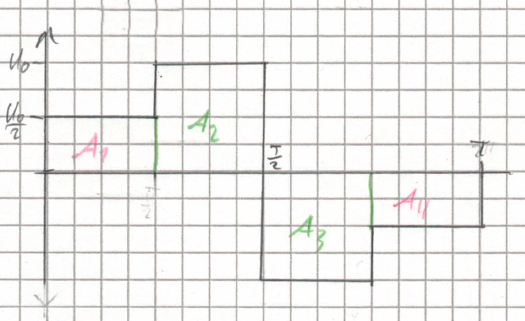
\includegraphics[width=.9\linewidth]{../../img/aufg6-a}
    \end{center}
\end{figure}


\begin{equation*}
    \begin{split}
        \bar{u} &= \frac{1}{T} \int_{t=t\cind{0}}^{t\cind{0} + T} u(t) dt\\
        \bar{u} &= \frac{A}{T}\\
        T &= 2 \pi\\
        \\
        A\cind{1} &= \frac{U\cind{0}}{2} * (\frac{\pi}{2} - 0\pi) &&= \frac{U\cind{0}}{2} * \frac{\pi}{2}\\
        A\cind{2} &= U\cind{0} * (\pi - \frac{\pi}{2}) &&= U\cind{0} * \frac{\pi}{2}\\
        A\cind{3} &= -\frac{U\cind{0}}{2} * (\frac{3\pi}{2} - \pi) &&= -\frac{U\cind{0}}{2} * \frac{\pi}{2}\\
        A\cind{4} &= -U\cind{0} * (2\pi - \frac{3\pi}{2}) &&= -U\cind{0} * \frac{\pi}{2}\\
        \\
    \end{split}
\end{equation*}

\[\bar{u} = \frac{ ( \frac{U\cind{0}}{2} * \frac{\pi}{2} ) + (U\cind{0} * \frac{\pi}{2}) + (-\frac{U\cind{0}}{2} * \frac{\pi}{2}) + (-U\cind{0} * \frac{\pi}{2}) }{2\pi} = 0\]

\newpage

\subsection*{b) - Effektivwert}

\begin{figure}[H]
    \begin{center}
        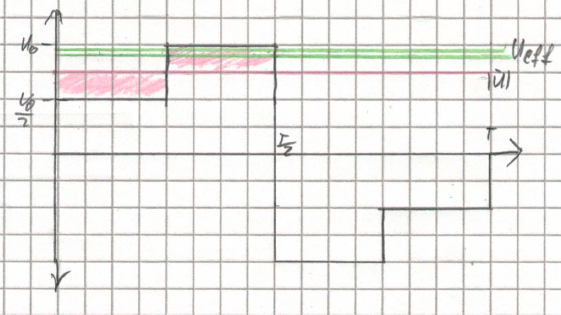
\includegraphics[width=.9\linewidth]{../../img/aufg6-b}
    \end{center}
\end{figure}

\emph{Für Pulssignale gilt:}

\[U\cind{eff} = \hat{u} * \sqrt{D}, D = \frac{t\cind{on}}{T}, \hat{u} = U\cind{0}\]

\begin{equation*}
    \begin{split}
        U\cind{eff} &= \sqrt{\frac{1}{T} \int_{t=t\cind{0}}^{t\cind{0} + T} u(t)^2 dt}\\
        D &= \frac{\frac{t\cind{on}}{2} + t\cind{on} + \frac{t\cind{on}}{2} + t\cind{on}}{T}\\
        &= \frac{3t\cind{on}}{T}\\
        U\cind{eff} &= U\cind{0} * \sqrt{\frac{3t\cind{on}}{T}}\\
    \end{split}
\end{equation*}

\subsection*{c) - Gleichrichtwert}

\begin{equation*}
    \begin{split}
        \left\lvert \bar{u} \right\rvert &= \frac{1}{T} \int_{t=t\cind{0}}^{t\cind{0} + T} \left\lvert u (t) \right\rvert  dt\\
        \bar{u} &= \frac{ \left\lvert A \right\rvert }{T}\\
        \left\lvert \bar{u} \right\rvert &= \frac{ \left\lvert A\cind{1} \right\rvert + \left\lvert A\cind{2} \right\rvert + \left\lvert A\cind{3} \right\rvert + \left\lvert A\cind{4} \right\rvert }{ T }\\
        &= \frac{3}{4} U\cind{0}
    \end{split}
\end{equation*}

\end{document}